% Adapted from the official CSC311 Fall 2026 report template.
% Proposal milestone: completed Data Exploration and planned Methodology only.
\documentclass[12pt]{article}
\usepackage[margin=1in]{geometry}
\usepackage{parskip,graphicx,booktabs,amsmath,amssymb}
\usepackage[hidelinks]{hyperref}
\usepackage{caption,enumitem}
\usepackage{lmodern}
\usepackage{fancyhdr}
\pagestyle{fancy}
\setlength{\headheight}{14.5pt}
\setlength{\emergencystretch}{2em}
\fancyhf{}
\fancyhead[L]{CSC311 Project Proposal}
\fancyhead[R]{\small MarkUs group\_62629}
\fancyfoot[C]{\thepage}
\captionsetup{font=small,labelfont=bf}
\setlist[itemize]{noitemsep,topsep=2pt,leftmargin=*}
\begin{document}
\begin{titlepage}
\centering
\vspace*{2.5cm}
{\Large CSC311: Introduction to Machine Learning\par}
\vspace{1cm}
{\LARGE Project Proposal\par}
\vspace{.6cm}
{\large Classifying Sports from Survey Responses\par}
\vspace{2cm}
{\large Submitted by\par}
\vspace{.5cm}
{\large MarkUs group\_62629\par}
\vspace{.5cm}
{\large Sixuan Song, Yuzhou Wu, Zhihan Fan, Junde Yang\par}
\vfill
{\large University of Toronto\\Fall 2026\par}
\end{titlepage}
\setcounter{page}{1}

\section{Data Exploration}
\textbf{Task and partition.}
The task is to classify a survey response as Baseball, Basketball, or Soccer. The
released file has 870 rows, 290 respondent IDs, 12 input questions, and a label.
We shuffled the sorted IDs with NumPy's generator (seed 311), reserved the first
44 IDs for a local test set and the next 44 for validation, and used the remaining
202 for training. The resulting row counts are 132/132/606, respectively.
All statistics, plots, vocabulary fitting, and feature--label analyses below use
only the 606 training rows. Each class has 202 training rows (33.3\%), so a constant
class predictor has 33.3\% training accuracy; class weighting or resampling is not
currently warranted. The row-level split manifest is included with the code.
The ID is a grouping key, never a model input. The local test set is separate
from the instructors' unreleased test set.

\begin{table}[h!]
\centering\small
\setlength{\tabcolsep}{4pt}
\begin{tabular}{@{}p{.74in}p{.68in}rrp{3.15in}@{}}
\toprule
Input & Type & Raw\% & Used\% & Training distribution / representation\\
\midrule
Ease & Numeric & 0 & 0 & Median 5, IQR 3--7, range 0--10\\
Strategy & Ordinal & 0 & 0 & Median 4, IQR 3--4; all five levels present\\
Injury & Ordinal & 0 & 0 & Median 4, IQR 3--4; all five levels present\\
Individual & Ordinal & 0 & 0 & Median 4, IQR 3--4; all five levels present\\
Venue & Multi-select & 0 & 0 & 7 distinct options; 58 response combinations\\
Season & Multi-select & 0 & 0 & 4 options; spring/summer/fall combination: 38.0\%\\
Music & Multi-select & 0 & 0 & 10 options; 91 response combinations\\
Food & Text & 2.64 & 2.64 & 449 distinct nonmissing strings; median 18 characters\\
Colour & Text & 0.99 & 0.99 & 146 distinct strings; median 5 characters\\
Song & Text & 10.56 & 10.56 & 330 distinct strings; median 19 characters\\
Feeling & Text & 0.50 & 0.50 & 345 distinct strings; median 10 characters\\
Price & Numeric text & 1.65 & 13.04 & Parsed median 100, IQR 50--225, range 0--10,000\\
\bottomrule
\end{tabular}
\caption{Every input feature. Raw\% is the normalized missing-response rate;
Used\% additionally includes failed numeric parsing. Text lengths and distinct
strings exclude normalized missing responses; each denominator for missingness is 606.}
\end{table}

\textbf{Quality checks and decisions.}
Case and whitespace vary, monetary answers mix symbols, prose, ranges, and currencies,
and some text contains staff-inserted redaction placeholders. We normalize Unicode,
case, and whitespace; empty strings, \texttt{n/a}, \texttt{none}, \texttt{-}, and
other explicit unknown markers mean no usable response. Their missingness is kept
as a feature. No training rows are exact duplicates across all inputs and the label.
No original input is constant: even the most common ordinal level is below 48\%.
The largest absolute off-diagonal numeric Spearman correlation is 0.31
(strategy/injury), so we retain both; their overlap does not justify deleting either.

\clearpage
\textbf{Feature--label relationships.}
Figure~\ref{fig:relationships} shows why both structured and textual responses are
useful. Baseball's ease mean is 4.02 (SD 2.05), versus 6.03 (2.12) for Basketball
and 6.16 (2.35) for Soccer. Individual-brilliance means are 3.73, 3.62, and 2.92,
respectively; substantial within-class spread prevents a single deterministic cutoff.
Indoor venue selection differs sharply: 23.3\%/96.5\%/63.4\% in the same class order.
Winter and hip-hop selections also distinguish Basketball.

\begin{figure}[h!]
\centering
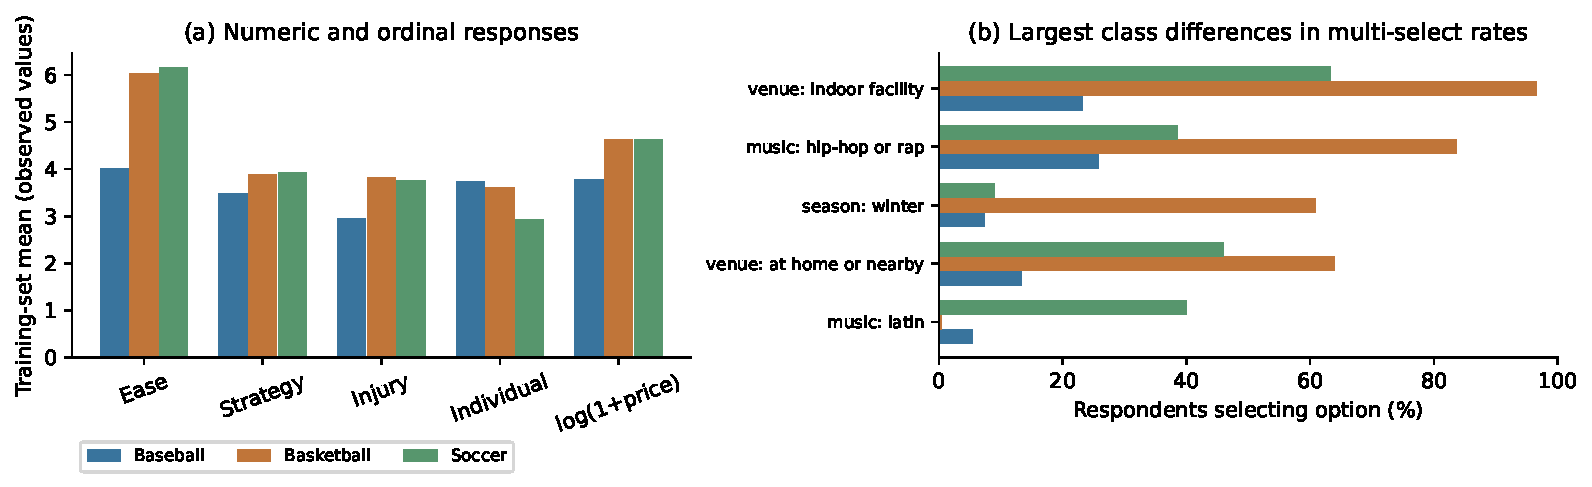
\includegraphics[width=\linewidth]{analysis/relationships.pdf}
\caption{Training-only associations. Numeric means exclude missing values; price
uses $\log(1+x)$ without the later model cap. Multi-select rates use all 202 rows
per class. The five options shown have the largest between-class rate ranges.}
\label{fig:relationships}
\end{figure}

Token presence, measured within each text field, provides additional signals.
``Green'' occurs in 3.0\%/0\%/55.0\% of colour responses, while ``orange'' occurs in
2.0\%/52.0\%/0.5\%. In songs, ``waka'' occurs in 50.0\% of Soccer rows and neither
other class; ``take me'' occurs in 29.2\% of Baseball rows only. In food, ``peanuts''
occurs in 12.4\%/0.5\%/0.5\%; in feelings, ``bored'' occurs in 27.2\%/5.4\%/8.9\%.
These exploratory associations motivate retaining all four text fields; they
are not validation scores. Complete distributions and association tables are
reproducible from the code and supplied in \texttt{analysis/}.

\textbf{Missingness and outliers.}
Song missingness differs by class (15.8\%/11.9\%/4.0\%), suggesting that an explicit
missing indicator may help. This does not identify whether responses are missing
at random. Price parsing accepts plain amounts and simple ranges (using their
midpoint), recognizes explicit unwillingness as zero, and abstains on ambiguous
prose, reversed ranges, and foreign currencies. Bare ``none'' remains missing.
This conservative rule leaves 79/606 prices unusable rather than inventing values.
The parsed distribution is right-skewed: mean 226.50 versus median 100, with 67
observations beyond the training 1.5-IQR fences. Large values may be genuine, so
we retain rows and cap price at the training 99th percentile (1,870), then apply
$\log(1+x)$. One ease response is 3.5; it is within the stated range and is retained.

Ordinal scores, multi-hot selections, and field-specific TF--IDF produce 1,389
columns for 606 rows at 2.24\% density. This high feature-to-row ratio supports
regularization and constrained model capacity. All fitted transformations are
re-estimated inside each training fold.

\clearpage
\section{Planned Methodology}
This section specifies the model-development plan. Data exploration and the
preprocessing implementation are complete. Compatibility checks have fitted each
model on one internal training fold; full tuning, validation comparison, and test
evaluation have not been run. No best-model or test-accuracy claim is made here.

\subsection*{Input representation and preprocessing}
All three model families use the same input questions. Our preprocessing
transformer learns its state only in \texttt{fit};
\texttt{transform} reuses that state. Placing it inside a scikit-learn pipeline
prevents the validation fold from determining imputation values, price caps,
scales, or vocabularies \cite{sklearnpitfalls}.

Ease is parsed as a number in $[0,10]$. The three Likert inputs map Strongly
disagree through Strongly agree to 1 through 5. This preserves order with one
coordinate, but assumes equal spacing; one-hot encoding would avoid that
assumption at the cost of more parameters. Our primary plan keeps the ordinal
encoding. For price, the rules and cap described above are applied, followed by
the log transform. Missing numeric values receive the median of that transformed
feature in the fitting partition; an entirely missing feature receives zero.
We then standardize each numeric coordinate with that partition's mean and
population standard deviation. Standardization gives zero mean and unit variance;
min--max scaling instead maps the observed minimum and maximum to fixed endpoints
and is more directly affected by extreme observations.

Each multi-select field receives a separate multi-hot vocabulary learned from
the fitting rows. We split on commas, normalize each option, and remove repeated
selections. ``No particular type'' remains a meaningful music option. Unseen
options are ignored rather than creating new columns. Each of the 12 raw input
fields also has an effective-missingness indicator (including numeric parse
failure), so imputation and empty text do not erase that information.

For food, colour, song, and feeling, we remove bracketed redactions and fit a
separate TF--IDF vectorizer with word unigrams and bigrams, Unicode accent stripping,
tokens of at least two characters, and no stop-word list or stemming. Each field
is capped at 500 terms and L2-normalized independently. With $n$ fitting documents,
the unnormalized weight is
\[
 (1+\log \mathrm{tf}_{t,d})
 \left[1+\log\frac{1+n}{1+\mathrm{df}_t}\right]
 \quad\text{when }\mathrm{tf}_{t,d}>0.
\]
This retains distinctive phrases while reducing repeated and ubiquitous words
\cite{sklearntext}. Unknown words produce no learned coordinate. Empty or
out-of-vocabulary responses give a zero text block; an empty fitted vocabulary is
handled without crashing. Numeric scaling matters for distance, gradient-based
optimization, and the relative effect of L2 regularization. It does not change
tree threshold ordering. Binary indicators and TF--IDF blocks remain unstandardized.

\clearpage
\subsection*{Model families and training}
We will compare the following three distinct families, using scikit-learn
implementations and the same respondent folds. Their statistical tradeoffs follow
the supervised-learning framework in \cite{hastie2009esl}.

\textbf{Multiclass softmax regression.}
Additive evidence across colour, song, and food terms makes a regularized linear
classifier a strong starting point. It is relatively interpretable and suitable
for sparse features. We will minimize multinomial cross-entropy with L2
regularization using L-BFGS, a maximum of 3,000 iterations, and tolerance $10^{-5}$.
The inverse regularization strength $C$ controls capacity. This solver uses no
learning-rate schedule or early stopping; convergence warnings must be resolved
before interpreting comparisons, increasing the iteration limit if necessary.

\textbf{Random forest.}
Venue, season, and numeric responses may interact nonlinearly; a forest can
represent threshold rules without assuming a linear decision boundary. We will
use 200 bootstrap-sampled CART trees with Gini impurity and seed 311, tuning depth,
minimum leaf size, and the feature subset per split. Bagging reduces variance,
while depth and leaf limits constrain overfitting. Training is greedy tree
construction, so there is no gradient optimizer or learning-rate schedule.

\textbf{K-nearest neighbours.}
The course baseline motivates testing a local-similarity model. We will use
brute-force neighbour search on the processed sparse features, comparing Manhattan
and Euclidean distance with uniform or inverse-distance voting. KNN has no
iterative training optimizer; the number of neighbours controls smoothing.
High dimension can make distances less informative, and numeric block scaling
can affect neighbour rankings, so this model is a useful contrasting hypothesis,
not an assumed winner. Large neural networks or language-model fine-tuning would
add substantial capacity relative to the 202 independent training respondents.

\begin{table}[h!]
\centering\small
\begin{tabular}{@{}p{.83in}p{5.45in}@{}}
\toprule
Family & Initial hyperparameter grid (24 candidates per family)\\
\midrule
Softmax & $C\in\{0.001,0.01,0.1,1,10,100\}$; minimum document frequency
$\in\{1,2,3,5\}$ for all four text vectorizers\\[4pt]
Forest & Maximum depth $\in\{3,6,12,\text{unlimited}\}$; minimum samples per leaf
$\in\{1,3,8\}$; split feature subset $\in\{\sqrt{p},0.3p\}$\\[4pt]
KNN & $k\in\{3,5,9,15,25,41\}$; weights $\in\{\text{uniform},\text{distance}\}$;
Minkowski exponent $\in\{1,2\}$\\
\bottomrule
\end{tabular}
\caption{Defaults held fixed: at most 500 terms per text field, word (1,2)-grams,
and minimum document frequency 2 except where tuned for softmax. $p$ is the
processed feature count. No family is selected before its tuning is complete.}
\end{table}

The logarithmic $C$ grid covers weak through strong regularization; text frequency
cutoffs trade rare phrases against variance. Forest settings span shallow to
unconstrained trees and progressively larger leaves. Odd $k$ values span very
local to smoother voting and remain below every fold's training size. All runs
use one computational worker for reproducibility. These grids are starting
budgets, not evidence that every useful value has been searched.

\clearpage
\subsection*{Validation, comparison, and final evaluation}
\textbf{Cross-validation.}
On the 606 training rows we will run five-fold
\texttt{StratifiedGroupKFold} with shuffle enabled and seed 311, grouping by ID
\cite{sklearngroups}. Each respondent stays entirely in one fold. Each pipeline
is refitted from scratch on four folds and scored on the fifth; transformations
must not be fit on all 606 rows before cross-validation. The released validation
and local test partitions remain outside this search. The supplied
\texttt{models.py} implements the initial grid search for every family.

\textbf{Metrics.}
Our primary selection metric will be macro-F1, the unweighted mean of the three
class F1 scores, where $F1_c=2P_cR_c/(P_c+R_c)$ and precision/recall use the
one-versus-rest counts for class $c$. Undefined scores are set to zero. We will
also report accuracy, per-class precision and recall, and a confusion matrix
with rows=true class and columns=predicted class. Macro-F1 exposes failure on a
single sport even if accuracy is acceptable. Weighted-F1 instead weights each
class by its support and can conceal a minority-class failure; macro-F1 is the
preferred complement to accuracy, including if the hidden test class balance
differs. A constant predictor on our balanced training data has macro-F1 $1/6$,
despite its 1/3 accuracy.

\textbf{Search review and model selection.}
For every candidate we will retain training scores, mean held-out fold scores,
and fold standard deviations. A large train--fold gap suggests excessive capacity,
calling for stronger regularization, shallower trees, larger leaves, or larger
$k$. If a best setting lies at a meaningful search boundary, we will expand that
boundary using training-fold scores only before opening the validation results;
any extra grid and rationale will be recorded. The initial code does not automate
this judgment. Equal candidate counts provide a transparent initial budget, but
do not guarantee equally exhaustive searches across families.

After fixing each family's best training-CV configuration by mean macro-F1, we
will compare all three on the untouched 132-row validation set once. We will
select the highest validation macro-F1; within 0.01 of the highest, prefer softmax,
then KNN, then forest for easier deployment. Small differences relative to
fold variation will be described as inconclusive, not as proof of superiority.
We will inspect per-class errors and compare structured-only versus full-feature
ablations within training CV if additional representation changes are needed;
validation results will not become a repeated tuning loop.

\textbf{Test and deployment.}
Only after locking the model and preprocessing will we refit on training plus
validation and evaluate the local 132-row test set once. This gains fitting data
but leaves no independent validation set for further revisions. Its accuracy,
class metrics, and uncertainty across respondent groups will support the final
report's single-number projected hidden-test accuracy. Student-response validation
cannot eliminate distribution shift to TA/instructor responses. We will then
prepare the separate \texttt{pred.py} milestone, exporting parameters and
preprocessing state to use only the standard library, NumPy, and pandas, with no
network access. The exact model must pass the 10 MB and approximately 60
predictions/minute limits; the present proposal code is development code and
does not claim to be that restricted prediction submission.

\clearpage
\section*{References and assistance}
The report format and project-specific decisions follow the official report
template, its two guiding-question appendices, the project instruction document
(Section 3.3 and Tables 2/4), and the October 9 project announcement
\cite{courserequirements,coursetemplate,courseupdate}.

\textbf{AI assistance.}
OpenAI Codex assisted with implementing the analysis and preprocessing, drafting
this proposal, and checking numerical consistency and document layout. Quantities
in Data Exploration come from the supplied scripts; the methodology is a plan,
not a claim that full experiments have already been completed.

\begingroup
\renewcommand{\section}[2]{}%
\bibliographystyle{plain}
\bibliography{proposal_references}
\endgroup
\end{document}
